\chapter{Electro-Optical Calibration}\label{ch:ElectroOptical}

Here, we will derive a formula for the amount of power in the first diffraction order when applying a Ronchi grating onto the SLM.
As an example, we first consider a Ronchi grating with ones period $M=1$, shown in \cref{fig:OneGrating}.

\begin{figure}[h]
    \centering
    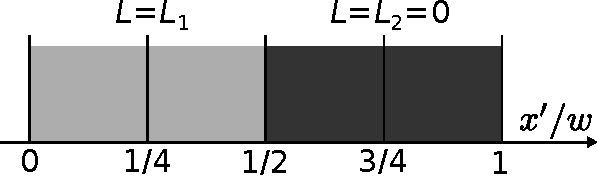
\includegraphics[width=0.42\textwidth]{figures/OneGrating.pdf}
    \caption{Ronchi grating for a single grating $M=1$ as well as $L_2=0$. The grating period $w$ is 8 pixels.}
    \label{fig:OneGrating}
\end{figure}

\noindent Assuming amplitude modulation between different gray levels is negligible (our new SLM has extremely low phase flicker), after applying the Ronchi grating of \cref{fig:OneGrating} the electric field just after the SLM will be

\begin{equation}\label{eq:Single}
    f(x,y) = e^{i\phi(L_1)} \operatorname{rect} \left\{ 
    \frac{x'-w/4}{w/2}\right\} +
    \operatorname{rect}\left\{ \frac{x'-3w/4}{w/2}\right\}.
\end{equation}
In \cref{eq:Single} $\operatorname{rect}\{(x'-a)/b\}$ is the rectangular function, which is unity for a width $b$ centered around $x'=a$ and zero elsewhere.
In the case of the single grating, $\{a=w/4, 3w/4\}$ and $b=w/2$.
For $M>1$, this pattern is simply repeated an additional $M-1$ times: \cite{Zhang1994}

\begin{equation}\label{eq:FieldAfterSLM}
    f(x,y) = \sum_{m=0}^{M-1} \left[
    e^{i \phi(L_1)} \operatorname{rect}\left\{\frac{x'-m w - w/4}{w/2}\right\} + 
    e^{i \phi(L_2)}\operatorname{rect}\left\{\frac{x'- m w - 3 w/4}{w/2}\right\}
    \right].
\end{equation}

\noindent According to Fourier optics, if we place a lens after the SLM, the field in the \textit{Fourier} plane of the lens is the 2D spatial Fourier transform of the field after the SLM, as derived in \cref{eq:FraunhoferDiffractionIntegral} as well as in \cref{eq:2Dcase}.
The field is thus for $y=0$ (we separate the different orders in the $x$-direction around $y=0$) proportional to the spatial Fourier transform $F = \mathcal{F}(f)$, and the intensity $I\propto |F|^2|$ as \cite{Zhang1994}

\begin{equation}\label{eq:FourierIntensity}
    |F(p,0)|^2\propto
    \frac{M^2 w^2}{2}\operatorname{sinc}^2\left(\frac{M p w}{2}\right) \times
    \frac{1 + \cos{\left[\phi(L)+p w/2\right]}}{\cos^2(p w/4)}.
\end{equation}
In \cref{eq:FourierIntensity} $p=2\pi x/\lambdaup f$ is the Fourier transformed spatial coordinate. 
The intensity in the first order ($p=\pm 2\pi/w$) is

\begin{equation}\label{eq:IntensityFirstOrderAppendix}
    I_1(\phi(L_1)) \propto
   w^2 \left[ 
    1-\cos{\phi(L_1)}
    \right].
\end{equation}
\Cref{eq:IntensityFirstOrderAppendix} is a usable expression for us because it relates the gray level $L_1$ to a measurable quantity $I_1$, which is the power in the first diffraction order. .